\documentclass[conference]{IEEEtran}

% ─── Packages ───────────────────────────────────────────────────────
\usepackage[utf8]{inputenc}
\usepackage[T1]{fontenc}
\usepackage{amsmath, amssymb, amsfonts}
\usepackage{graphicx}
\usepackage{booktabs}
\usepackage{cite}
\usepackage{hyperref}
\usepackage{caption}
\usepackage{subcaption}
\usepackage{float}
\usepackage{enumitem}
\usepackage{multirow}
\usepackage{array}
\usepackage[ruled,vlined]{algorithm2e}
\usepackage{xcolor}

\hypersetup{colorlinks=true, linkcolor=blue, citecolor=blue, urlcolor=blue}

% ─── Title ──────────────────────────────────────────────────────────
\title{Parkinson's Disease Detection from Bilateral Wrist-Worn Smartwatch IMU Data Using Dual-Channel Cross-Attention Transformers}

\author{
  \IEEEauthorblockN{Author Name}
  \IEEEauthorblockA{\\\
  University Name \\
  \texttt{author@email.edu}}
}

% ════════════════════════════════════════════════════════════════════
\begin{document}
\maketitle

% ─── Abstract ───────────────────────────────────────────────────────
\begin{abstract}

\end{abstract}

% ─── I. Introduction ───────────────────────────────────────────────
\section{Introduction}



The system addresses two classification problems in a hierarchical manner:
\begin{enumerate}[noitemsep]
  \item \textbf{HC vs PD}: Distinguishing Healthy Controls from Parkinson's Disease patients.
  \item \textbf{PD vs DD}: Differentiating PD patients from those with other Differential Diagnosis movement disorders.
\end{enumerate}

This hierarchical dual-head approach was chosen over a single three-class classifier because the clinical decision boundary between PD and DD is inherently more nuanced than the healthy-vs-diseased boundary.

% ─── II. Related Work ──────────────────────────────────────────────
\section{Related Work}

% ─── III. Dataset ──────────────────────────────────────────────────
\section{Dataset}

\subsection{Overview}
The PADS (Parkinson's Disease Smartwatch) dataset contains bilateral wrist-worn smartwatch recordings from $469$ participants performing $10$ standardised motor tasks.

\begin{table}[H]
\centering
\caption{Patient distribution by condition.}
\label{tab:patients}
\begin{tabular}{lc}
\toprule
\textbf{Condition} & \textbf{Count} \\
\midrule
Healthy Controls (HC)        & $79$  \\
Parkinson's Disease (PD)     & $291$ \\
Differential Diagnosis (DD)  & $99$  \\
\midrule
\textbf{Total Patients}      & \textbf{469} \\
\bottomrule
\end{tabular}
\end{table}

\subsection{Sensor Modality}
Each participant wears a smartwatch on both wrists, providing six-axis IMU measurements per wrist: three-axis accelerometer ($a_x, a_y, a_z$) and three-axis gyroscope ($\omega_x, \omega_y, \omega_z$), sampled at $100$~Hz.

\subsection{Motor Tasks}
Ten standardised motor tasks are recorded: \textit{CrossArms}, \textit{DrinkGlas}, \textit{Entrainment}, \textit{HoldWeight}, \textit{LiftHold}, \textit{PointFinger}, \textit{Relaxed}, \textit{StretchHold}, \textit{TouchIndex}, and \textit{TouchNose}. These tasks are designed to elicit different aspects of motor impairment associated with Parkinson's Disease.

\begin{figure}[H]
\centering

\includegraphics[width=0.45\textwidth]{image5.png}
\caption{Visualisation of the sensor data from patient tasks.}
\label{fig:sensor_viz}
\end{figure}

\subsection{Label Encoding}
The hierarchical labelling scheme assigns:
\begin{itemize}[noitemsep]
  \item HC samples: HC vs PD label $= 0$, PD vs DD label $= -1$ (masked).
  \item PD samples: HC vs PD label $= 1$, PD vs DD label $= 0$.
  \item DD samples: HC vs PD label $= -1$ (masked), PD vs DD label $= 1$.
\end{itemize}
Labels of $-1$ are masked during loss computation, ensuring each classification head is trained only on relevant samples.

\subsection{Train-Validation Split}
\label{sec:split}
A \textbf{patient-level stratified $5$-fold cross-validation} strategy is used. All windows from a given patient remain entirely within either the training or validation set, preventing data leakage.

\begin{table}[H]
\centering
\caption{Sample distribution across folds (patient-level stratified split).}
\label{tab:folds}
\begin{tabular}{ccccc}
\toprule
\textbf{Fold} & \textbf{Train Total} & \textbf{Train (HC/PD/DD)} & \textbf{Test Total} & \textbf{Test (HC/PD/DD)} \\
\midrule
1 & 25\,640 & 7\,938 / 8\,854 / 8\,848 & 6\,460 & 2\,016 / 2\,204 / 2\,240 \\
2 & 25\,640 & 7\,938 / 8\,854 / 8\,848 & 6\,460 & 2\,016 / 2\,204 / 2\,240 \\
3 & 25\,640 & 7\,938 / 8\,854 / 8\,848 & 6\,460 & 2\,016 / 2\,204 / 2\,240 \\
4 & 25\,714 & 7\,938 / 8\,816 / 8\,960 & 6\,386 & 2\,016 / 2\,242 / 2\,128 \\
5 & 25\,766 & 8\,064 / 8\,854 / 8\,848 & 6\,334 & 1\,890 / 2\,204 / 2\,240 \\
\bottomrule
\end{tabular}
\end{table}

% ─── IV. Methodology ──────────────────────────────────────────────
\section{Methodology}

\subsection{Data Preprocessing}

\subsubsection{Downsampling}
The raw signals are resampled from the native $100$~Hz to $64$~Hz using polyphase resampling, preserving the frequency content relevant to human motor movements (predominantly below $20$~Hz).

\subsubsection{Band-Pass Filtering}
A fourth-order Butterworth band-pass filter with passband $[0.1, 20]$~Hz is applied. The low-frequency cutoff at $0.1$~Hz removes DC offset and slow drift, while the high-frequency cutoff at $20$~Hz removes noise above the motor frequency range. The filter is applied using zero-phase forward-backward filtering to avoid phase distortion.

\subsubsection{Windowing with Differential Overlap Sampling}
\label{sec:windowing}
The continuous signals are segmented into fixed-length windows of \textbf{256 time steps}. At $64$~Hz, each window captures $4.0$ seconds of motor activity.

To address the \textbf{class imbalance} ($79$ HC vs $291$ PD vs $99$ DD), a \textbf{differential overlap sampling strategy} is employed:

\begin{table}[H]
\centering
\caption{Differential overlap sampling strategy for class balancing.}
\label{tab:overlap}
\begin{tabular}{lcc}
\toprule
\textbf{Condition} & \textbf{Overlap Ratio} & \textbf{Effective Step Size} \\
\midrule
HC  & $70\%$ & $0.30 \times 256 = 77$ samples \\
PD  & $0\%$  & $1.00 \times 256 = 256$ samples \\
DD  & $65\%$ & $0.35 \times 256 = 90$ samples \\
\bottomrule
\end{tabular}
\end{table}

This produces approximately balanced sample counts across conditions ($\sim 8{,}000$ per class in training; see Table~\ref{tab:folds}).

\subsection{Dual-Channel Cross-Attention Transformer}
\label{sec:base_model}

The primary model independently processes left and right wrist signals through parallel encoding streams, then fuses bilateral information via cross-attention. Fig.~\ref{fig:architecture} illustrates the architecture.

\begin{figure}[H]
\centering

\includegraphics[width=0.45\textwidth]{image1.png}
\caption{Dual-channel cross-attention Transformer architecture. Left and right streams are processed independently through projection, positional encoding, and cross-attention layers before pooling and concatenation for classification.}
\label{fig:architecture}
\end{figure}

\subsubsection{Input Projection}
Each wrist's 6-channel input $\mathbf{X} \in \mathbb{R}^{T \times 6}$ ($T = 256$) is linearly projected:
\begin{equation}
\mathbf{H}^{(0)} = \mathbf{X} \mathbf{W}_{\text{proj}} + \mathbf{b}_{\text{proj}}, \quad \mathbf{W}_{\text{proj}} \in \mathbb{R}^{6 \times d_{\text{model}}}
\end{equation}

\subsubsection{Sinusoidal Positional Encoding}
Sinusoidal positional encoding injects temporal ordering:
\begin{align}
\text{PE}(t, 2i)   &= \sin\!\left(\frac{t}{10000^{\,2i / d_{\text{model}}}}\right) \\
\text{PE}(t, 2i+1) &= \cos\!\left(\frac{t}{10000^{\,2i / d_{\text{model}}}}\right)
\end{align}

\subsubsection{Cross-Attention Layer}
Each cross-attention layer comprises four sub-stages per channel with residual connections and layer normalisation. Let $\mathbf{L}$ and $\mathbf{R}$ denote the left and right channel representations:
\begin{enumerate}[noitemsep]
  \item \textbf{Self-Attention}: $\mathbf{L}' = \text{LN}\!\bigl(\mathbf{L} + \text{MHA}(\mathbf{L}, \mathbf{L}, \mathbf{L})\bigr)$
  \item \textbf{Cross-Attention}: $\mathbf{L}'' = \text{LN}\!\bigl(\mathbf{L}' + \text{MHA}(\mathbf{L}', \mathbf{R}', \mathbf{R}')\bigr)$
  \item \textbf{Feed-Forward}: $\text{FFN}(\mathbf{x}) = \text{LN}\!\bigl(\mathbf{x} + \mathbf{W}_2 \cdot \text{ReLU}(\mathbf{W}_1 \mathbf{x} + \mathbf{b}_1) + \mathbf{b}_2\bigr)$
\end{enumerate}

\subsubsection{Global Pooling and Classification}
After $N$ cross-attention layers, global average pooling reduces the temporal dimension. The pooled representations are concatenated and fed into two independent classification heads:
\begin{equation}
\hat{y}_{\text{HC}} = \mathbf{W}_{\text{HC}} [\mathbf{z}_L \| \mathbf{z}_R] + \mathbf{b}_{\text{HC}}, \quad
\hat{y}_{\text{PD}} = \mathbf{W}_{\text{PD}} [\mathbf{z}_L \| \mathbf{z}_R] + \mathbf{b}_{\text{PD}}
\end{equation}

\subsubsection{Design Decision: Removal of Text Encoder}
An initial design incorporated a BERT-based text encoder for patient metadata fusion. However, the model was observed to shortcut by predicting primarily from metadata. The text encoder was removed to ensure the model learns discriminative features solely from the IMU data.

\subsection{Model Hyperparameters}

\begin{table}[H]
\centering
\caption{Base model hyperparameters.}
\label{tab:hyperparams}
\begin{tabular}{ll}
\toprule
\textbf{Parameter} & \textbf{Value} \\
\midrule
Input dimension (per wrist)     & $6$   \\
Model dimension                 & $128$ \\
Number of attention heads        & $8$   \\
Number of cross-attention layers & $4$   \\
Feed-forward hidden dimension   & $512$ \\
Dropout rate                     & $0.1$ \\
Sequence length                  & $256$ \\
\bottomrule
\end{tabular}
\end{table}

\subsection{Training Procedure}

\subsubsection{Objective Function}
The total loss is the average of two independent cross-entropy losses over valid samples:
\begin{equation}
\mathcal{L} = \frac{1}{|\mathcal{S}|} \sum_{s \in \mathcal{S}} \mathcal{L}_s, \quad
\mathcal{L}_s = -\sum_{c=1}^{2} y_{s,c} \log \hat{p}_{s,c}
\end{equation}
where $\mathcal{S}$ is the set of active classification heads (those with valid, non-masked labels).

\subsubsection{Optimisation}
AdamW optimiser with learning rate $5 \times 10^{-4}$, weight decay $0.01$, gradient clipping at unit norm. ReduceLROnPlateau scheduler halves the learning rate after $5$ epochs without improvement. Training: up to $100$ epochs, batch size $32$.

\subsubsection{Model Selection}
The combined validation accuracy (arithmetic mean of HC vs PD and PD vs DD accuracies) selects the best checkpoint.

% ─── V. Experiments and Results ────────────────────────────────────
\section{Experiments and Results}

\subsection{Base Model Evaluation}

The base model was trained with the hyperparameters in Table~\ref{tab:hyperparams} across five folds.

\begin{table}[H]
\centering
\caption{Initial model results with band-pass filtering (Fold~1, best epoch~77).}
\label{tab:base_results}
\begin{tabular}{lcccc}
\toprule
\textbf{Task} & \textbf{Accuracy} & \textbf{Precision} & \textbf{Recall} & \textbf{F1} \\
\midrule
HC vs PD & $96.11\%$ & $96.37\%$ & $96.11\%$ & $96.10\%$ \\
PD vs DD & $95.43\%$ & $95.80\%$ & $95.43\%$ & $95.42\%$ \\
\midrule
\textbf{Combined} & \multicolumn{4}{c}{\textbf{95.77\%}} \\
\bottomrule
\end{tabular}
\end{table}

\begin{figure}[H]
\centering
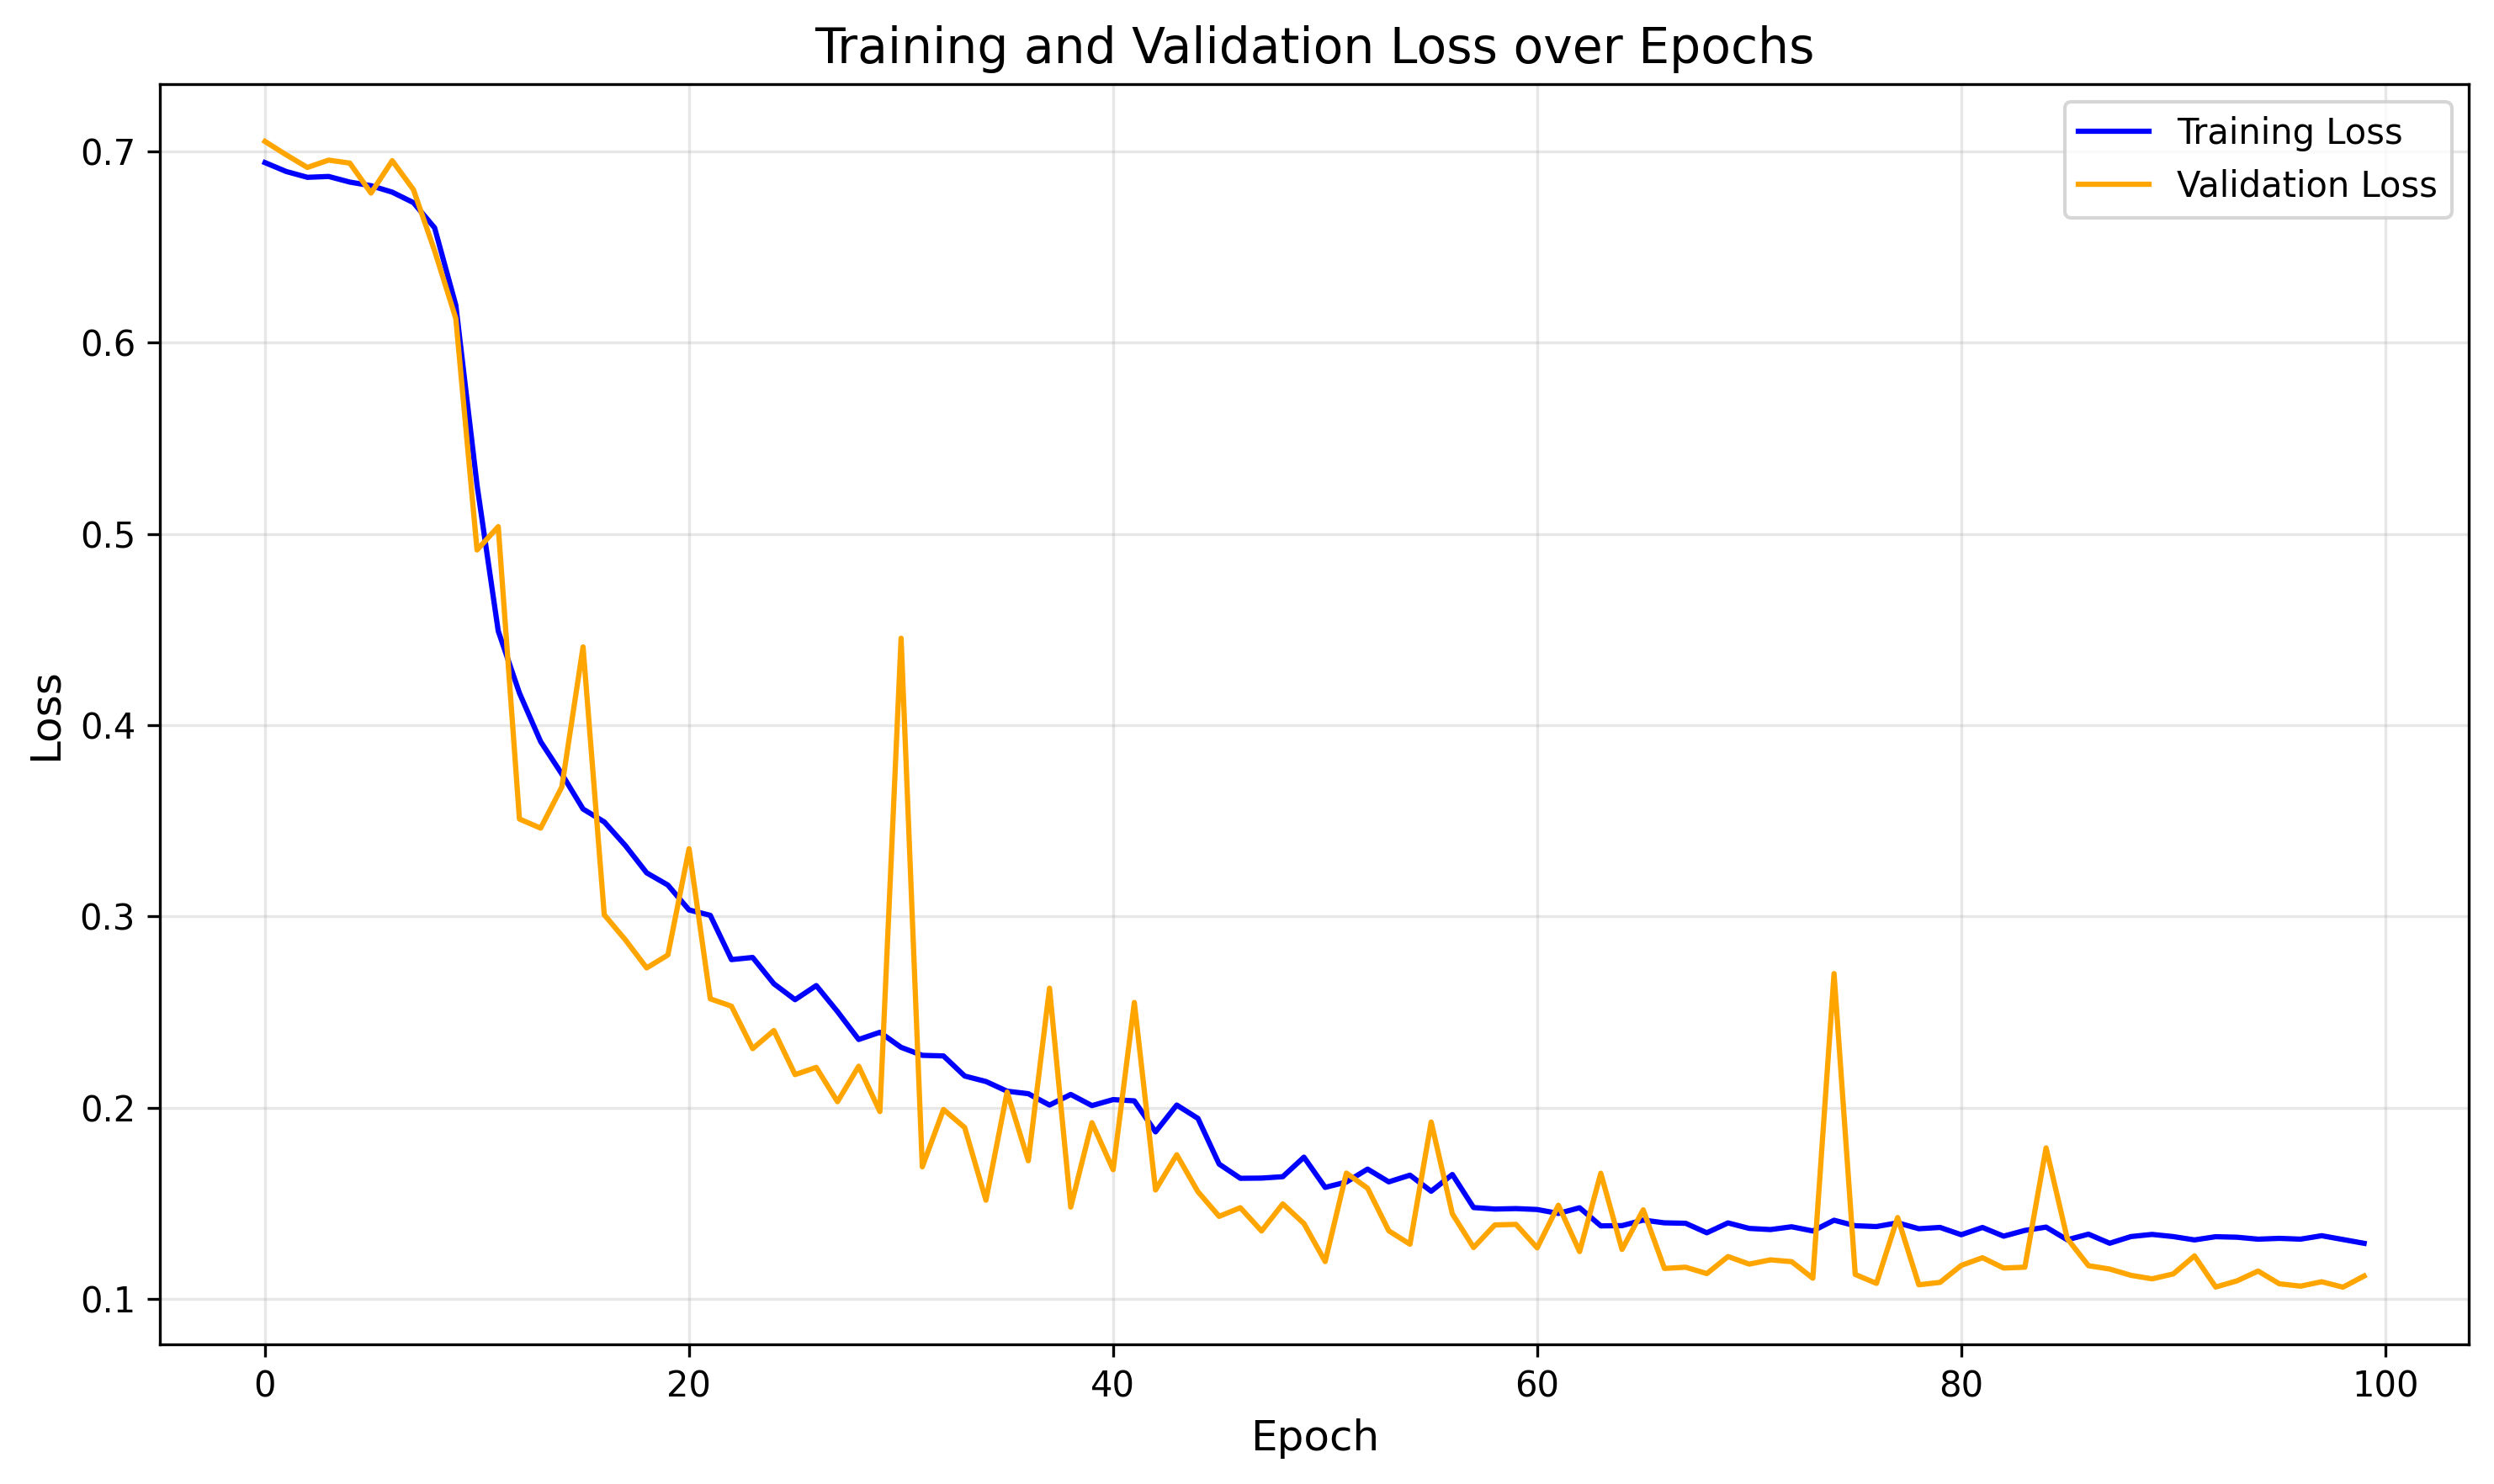
\includegraphics[width=0.45\textwidth]{results/Initial_model_with_bandpass/plots/fold_1/loss.png}
\caption{Training and validation loss over epochs for the initial model with band-pass filter (Fold~1).}
\label{fig:initial_loss}
\end{figure}

\begin{figure}[H]
\centering
\begin{subfigure}[b]{0.23\textwidth}
    \centering
    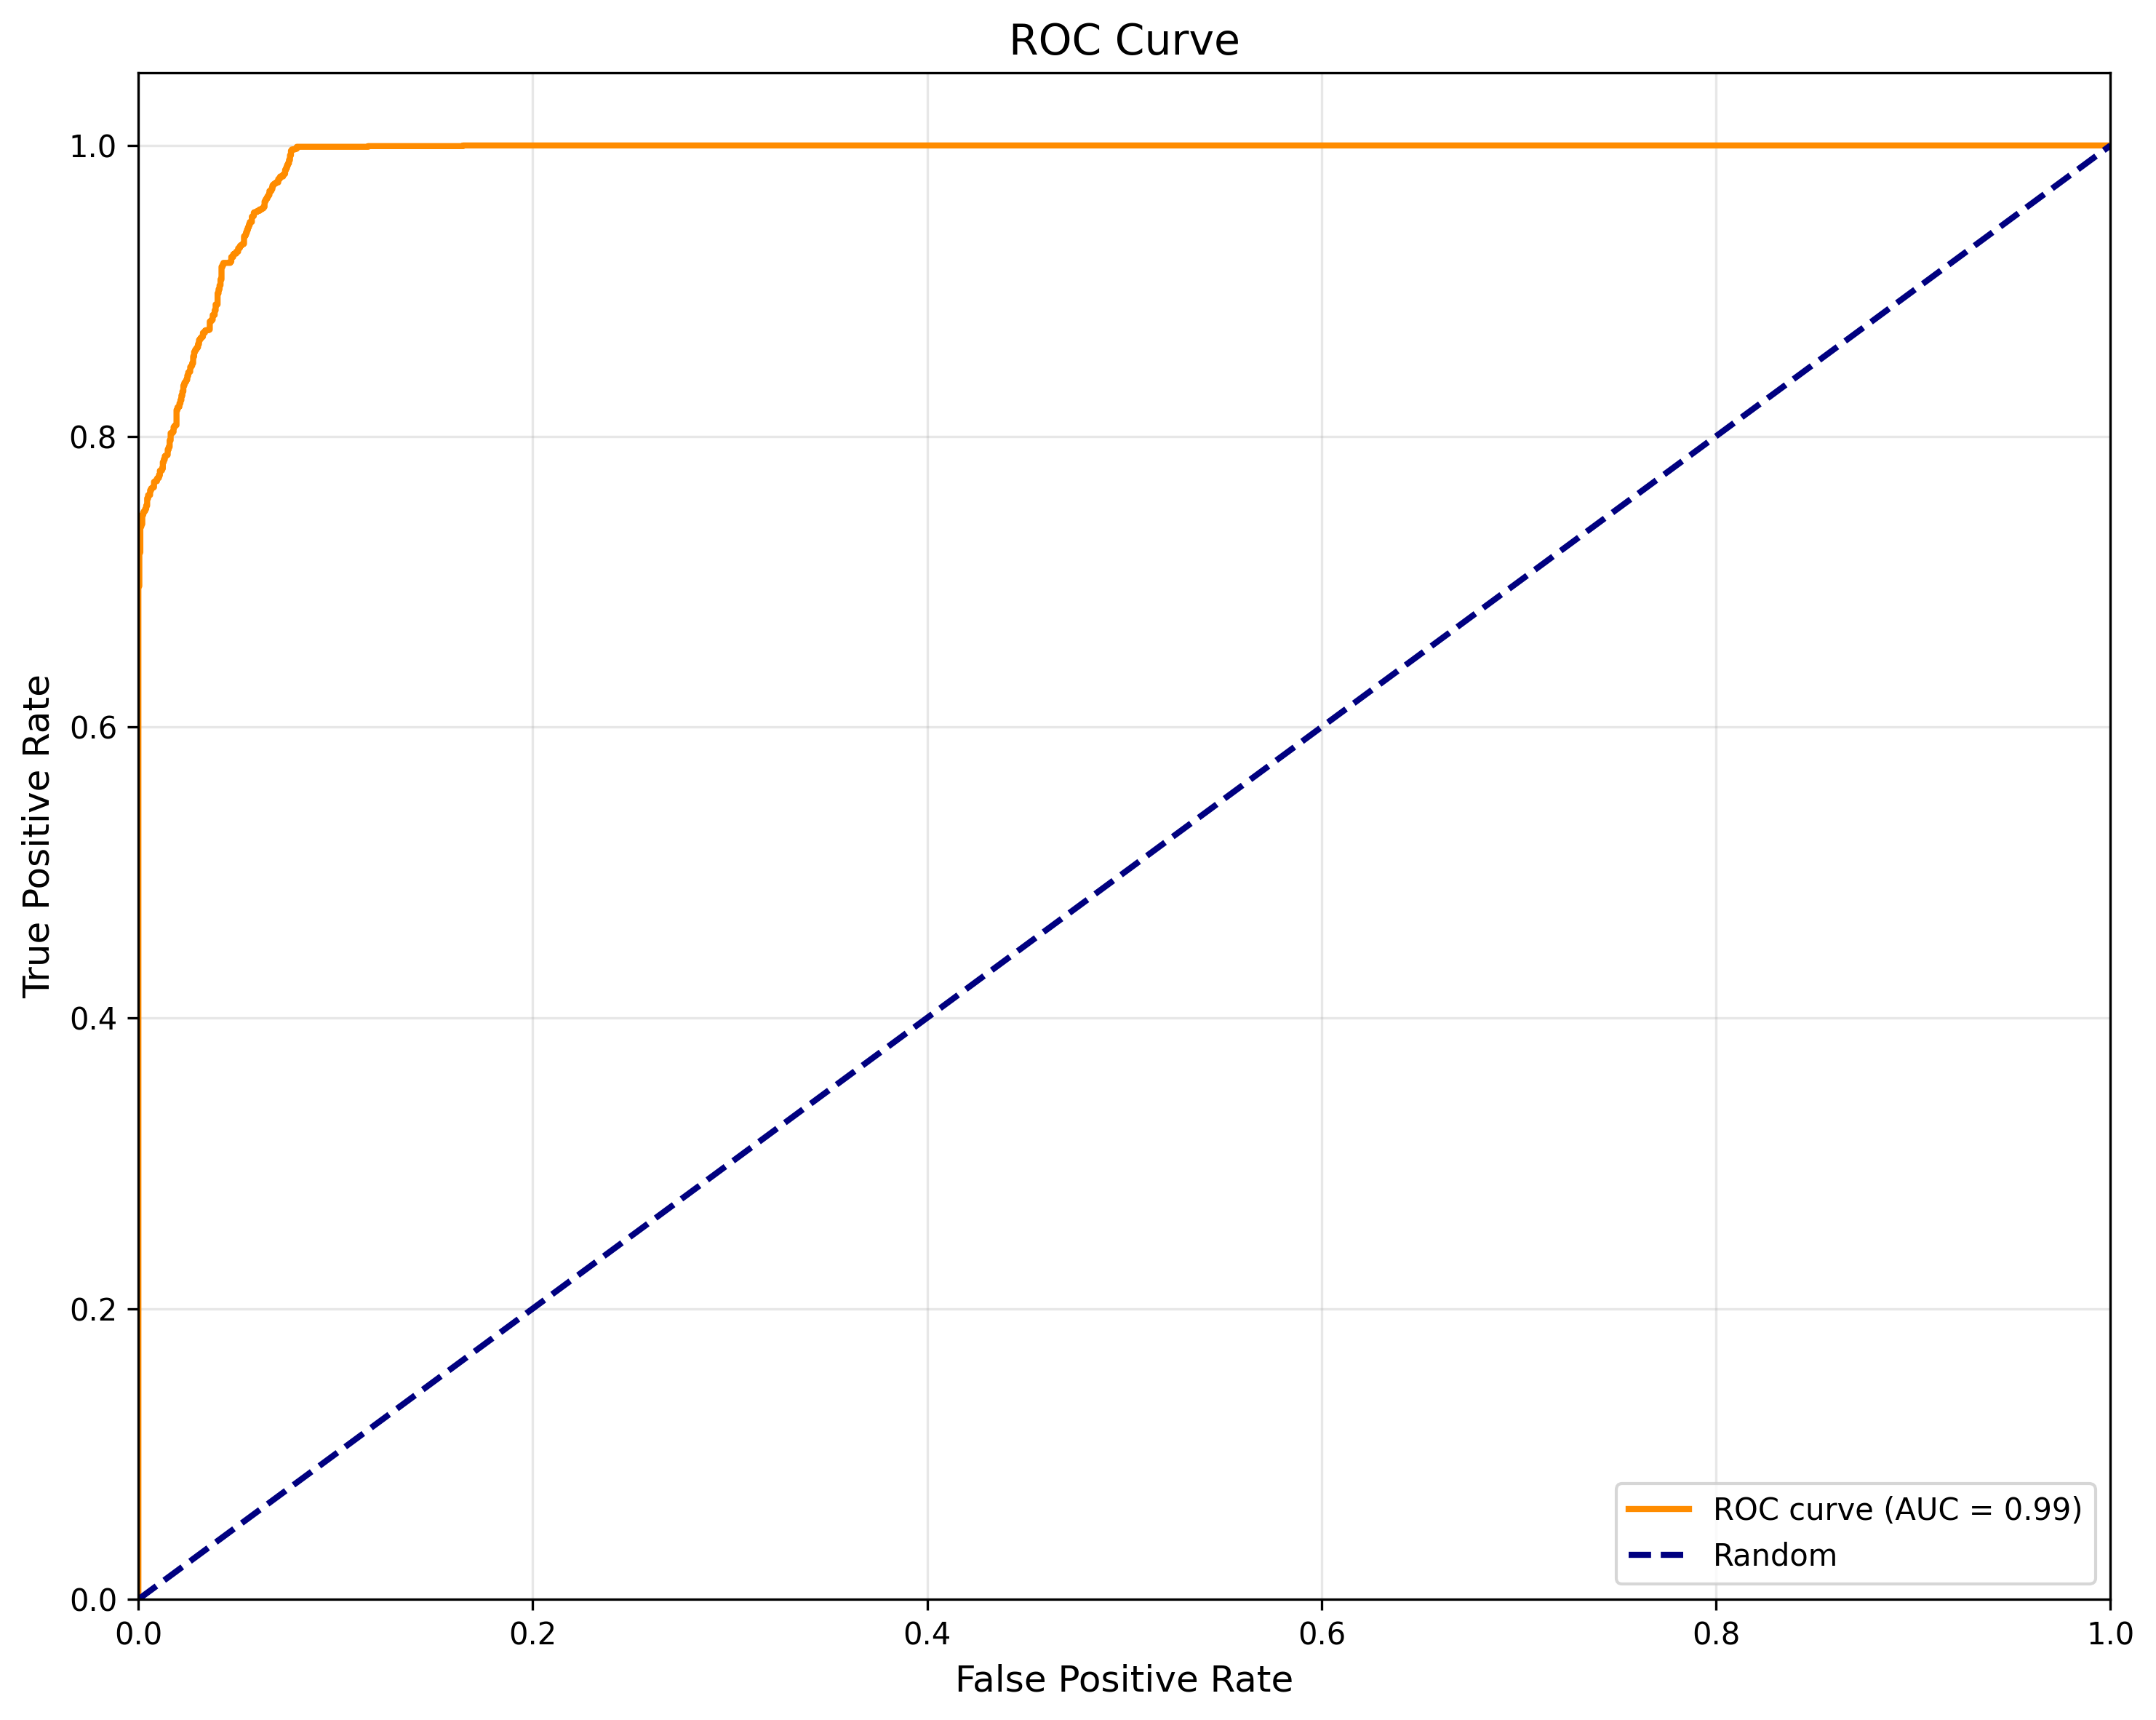
\includegraphics[width=\textwidth]{results/Initial_model_with_bandpass/plots/fold_1/roc_hc_vs_pd.png}
    \caption{HC vs PD ROC}
\end{subfigure}
\hfill
\begin{subfigure}[b]{0.23\textwidth}
    \centering
    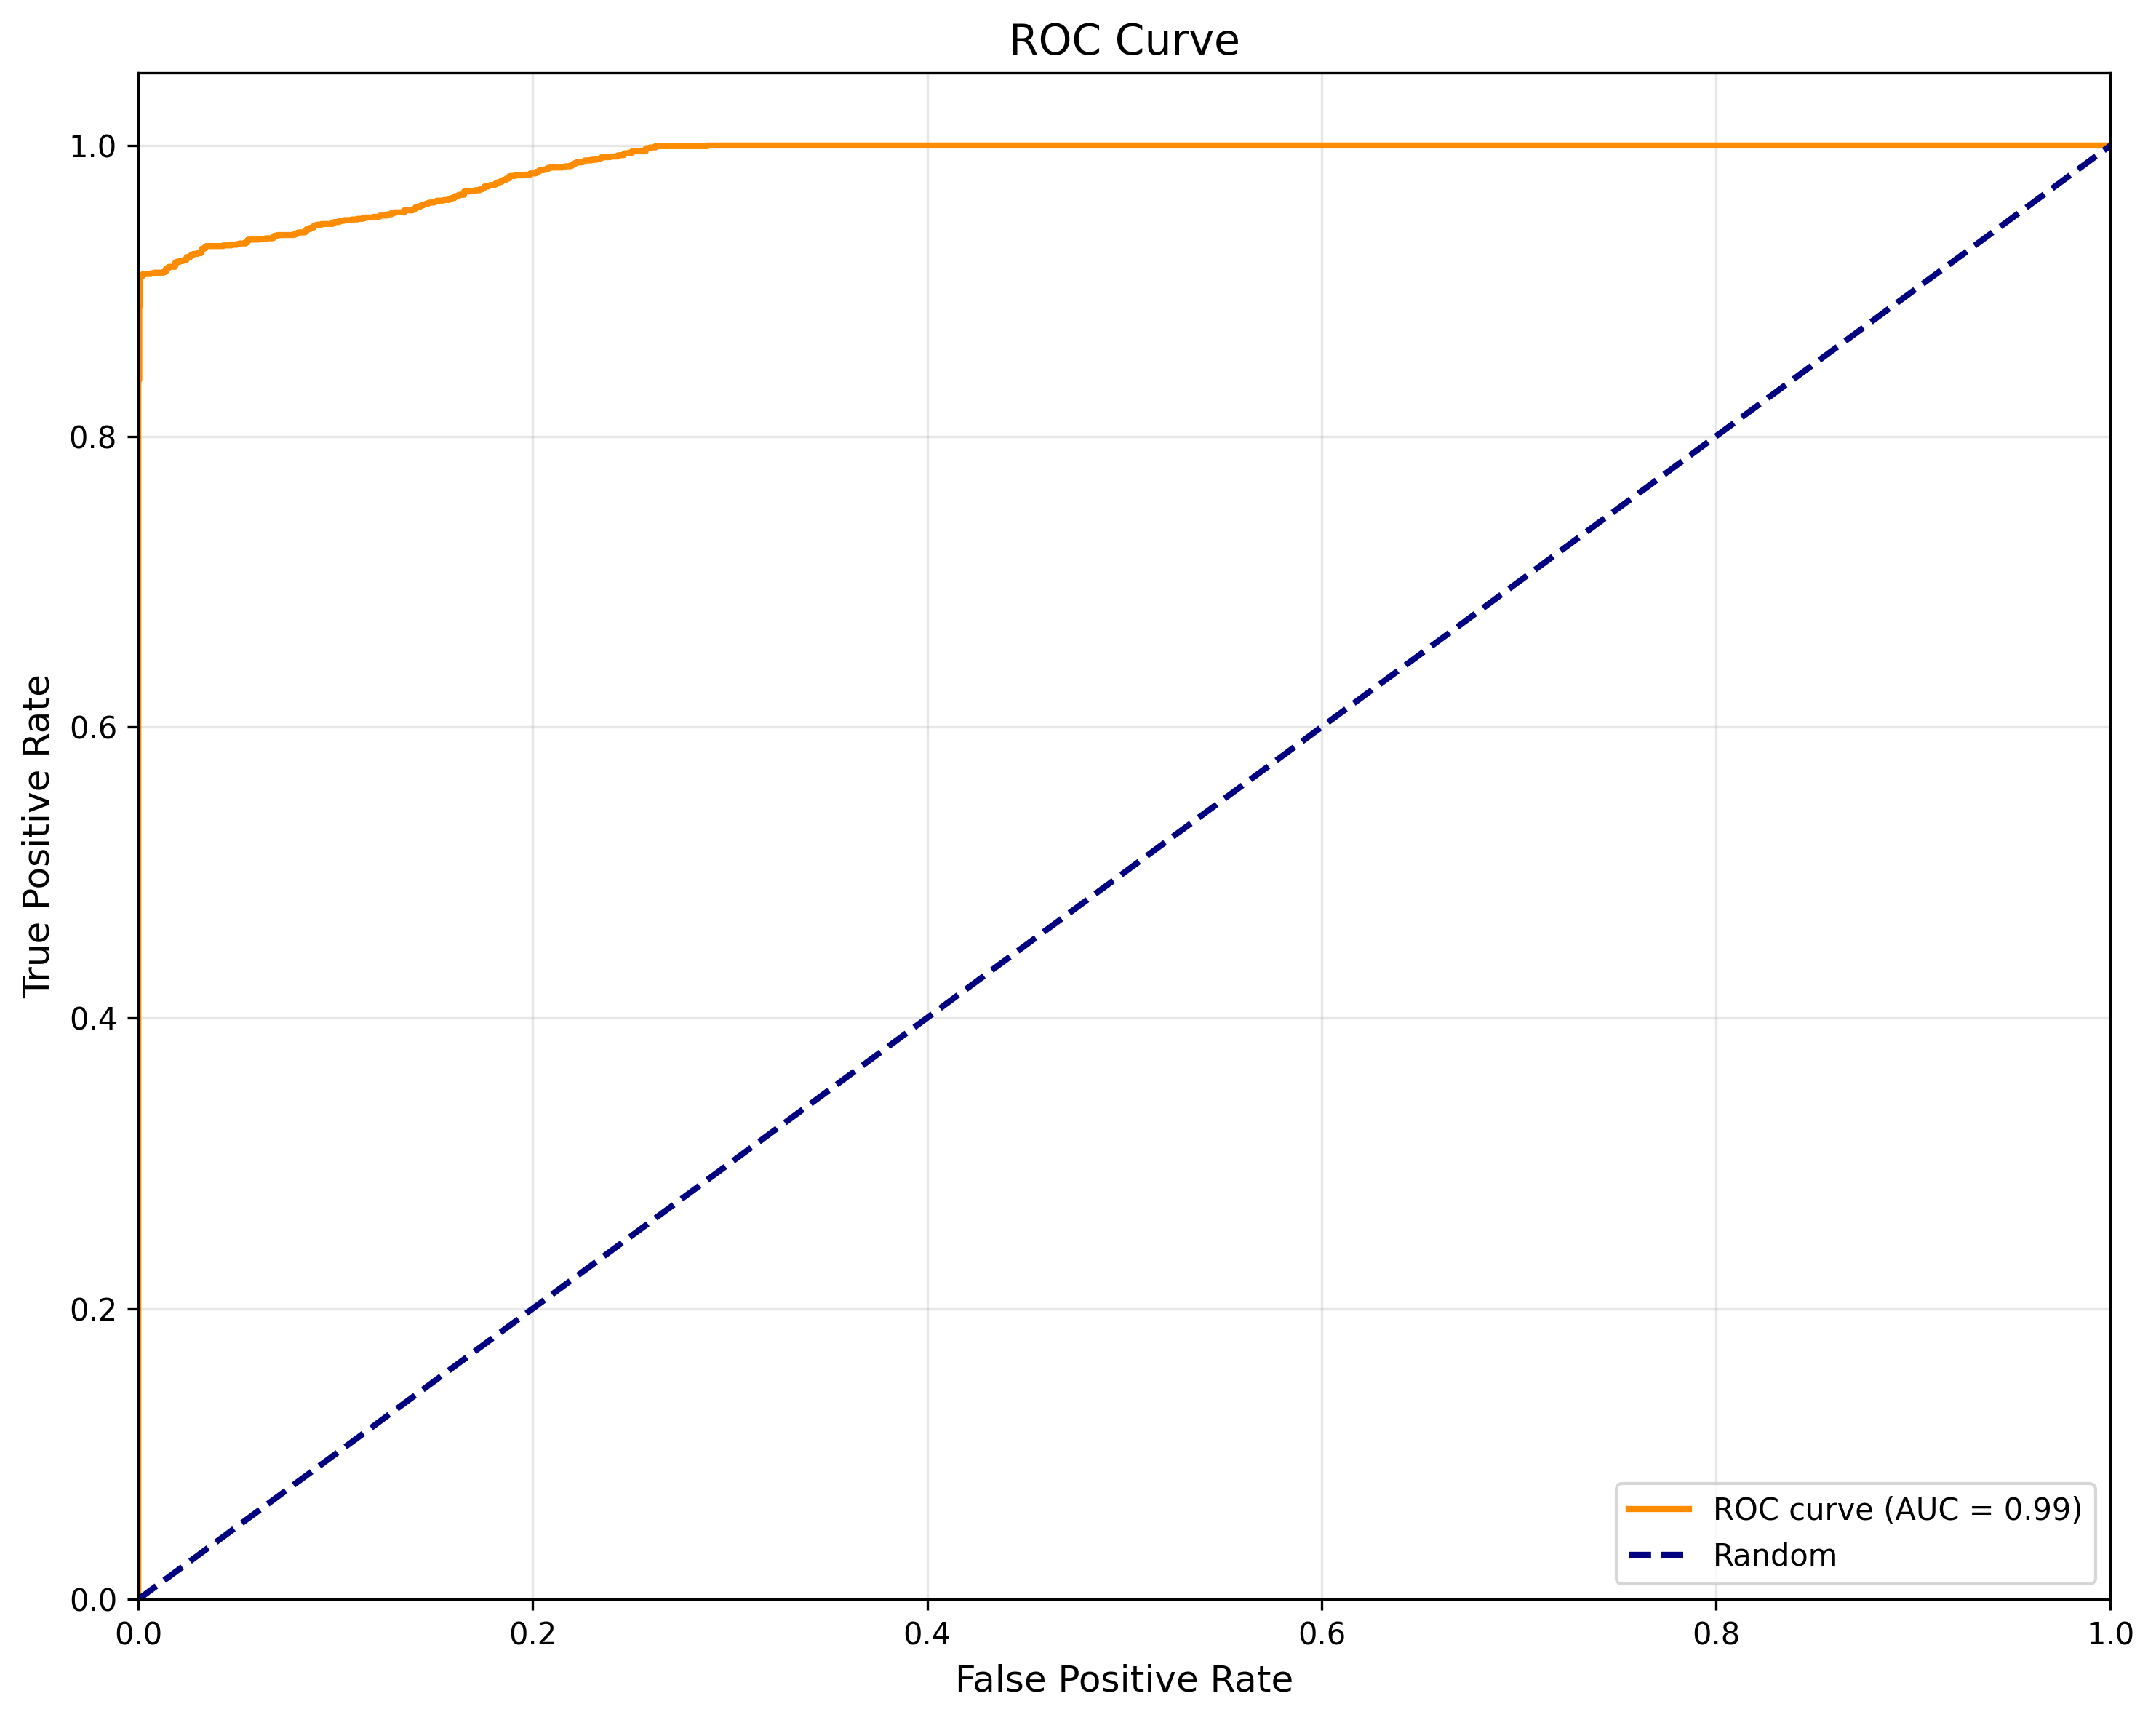
\includegraphics[width=\textwidth]{results/Initial_model_with_bandpass/plots/fold_1/roc_pd_vs_dd.png}
    \caption{PD vs DD ROC}
\end{subfigure}
\caption{ROC curves for the initial model with band-pass filter (Fold~1).}
\label{fig:initial_roc}
\end{figure}

\begin{figure}[H]
\centering
\begin{subfigure}[b]{0.23\textwidth}
    \centering
    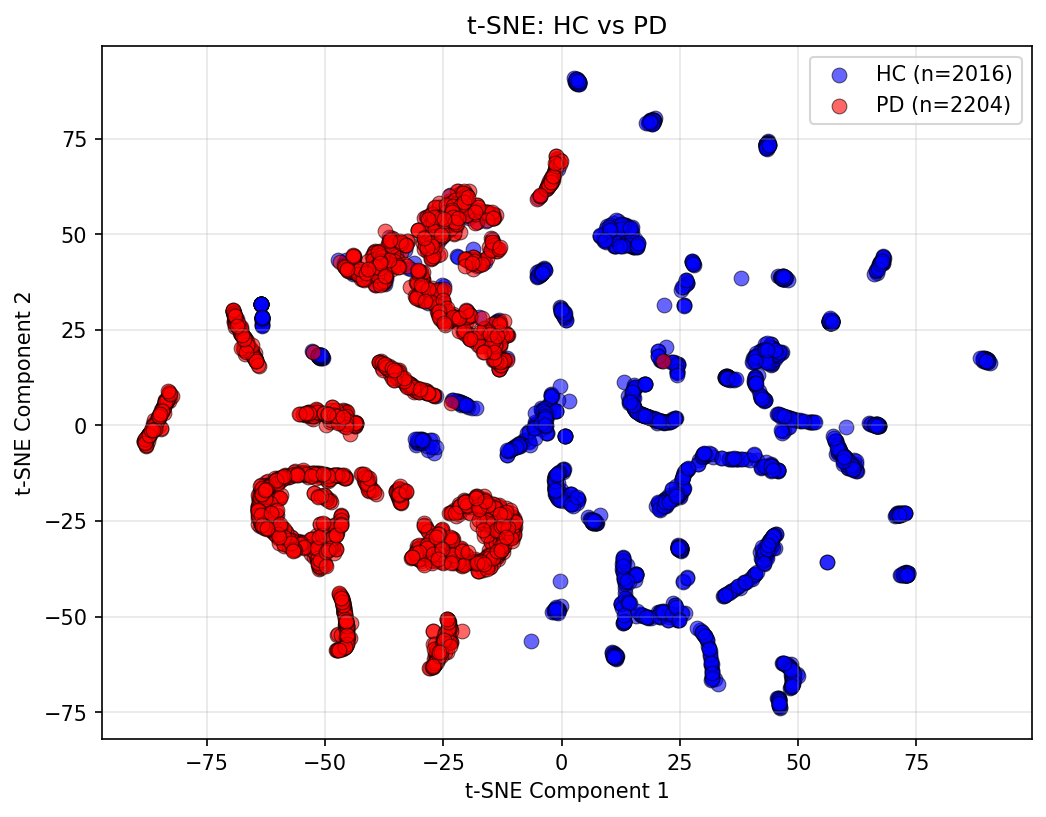
\includegraphics[width=\textwidth]{results/Initial_model_with_bandpass/plots/fold_1/tsne_hc_vs_pd.png}
    \caption{HC vs PD}
\end{subfigure}
\hfill
\begin{subfigure}[b]{0.23\textwidth}
    \centering
    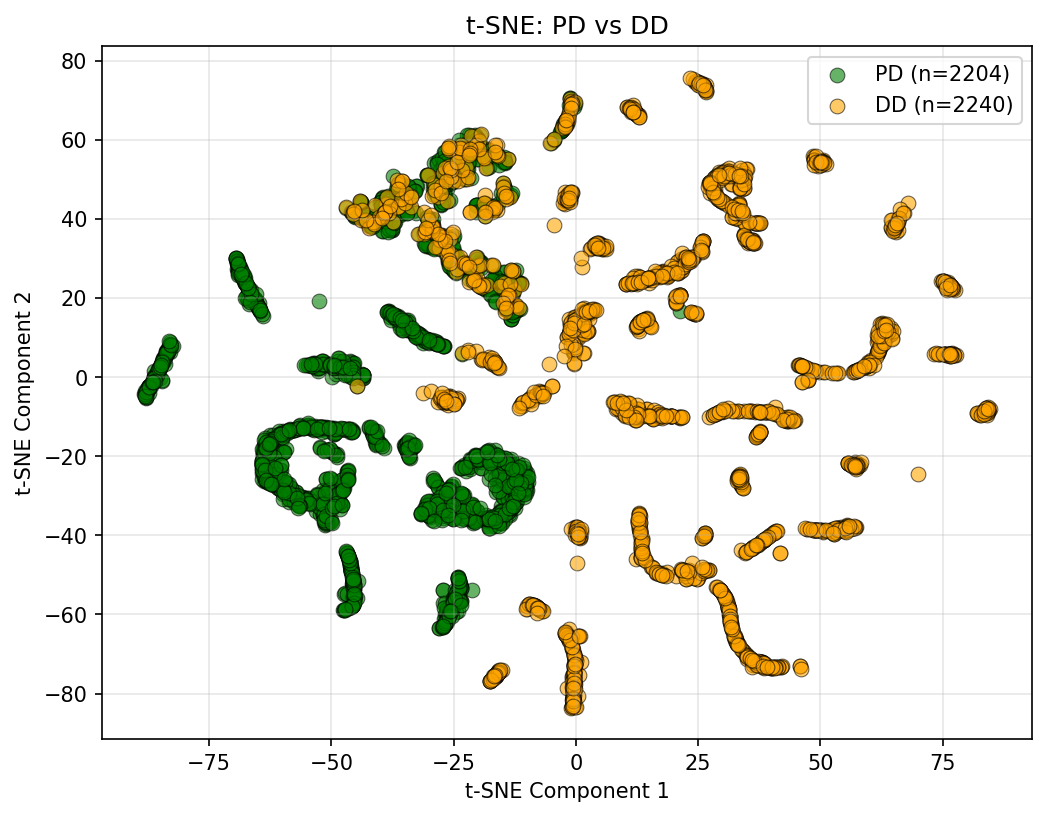
\includegraphics[width=\textwidth]{results/Initial_model_with_bandpass/plots/fold_1/tsne_pd_vs_dd.png}
    \caption{PD vs DD}
\end{subfigure}
\caption{t-SNE feature embeddings for the initial model with band-pass filter (Fold~1).}
\label{fig:initial_tsne}
\end{figure}


\subsection{Signal Preprocessing Ablation: Band-Pass Filtering}

To validate the importance of the band-pass filtering step, the Optuna-optimised model ($d_{\text{model}}{=}32$, $N{=}3$; see Table~\ref{tab:optuna_best}) was trained under two conditions: (a) with the $[0.1, 20]$~Hz Butterworth band-pass filter, and (b) without any frequency-domain filtering. All other hyperparameters are identical between the two runs.

\begin{table}[H]
\centering
\caption{Effect of band-pass filtering on base model performance (Fold 1).}
\label{tab:bandpass}
\begin{tabular}{lccc}
\toprule
\textbf{Variant} & \textbf{HC vs PD} & \textbf{PD vs DD} & \textbf{Combined} \\
\midrule
With band-pass    & $94.03\%$ & $94.21\%$ & $94.12\%$ \\
Without band-pass & $88.67\%$ & $88.32\%$ & $88.50\%$ \\
\bottomrule
\end{tabular}
\end{table}

\begin{figure}[H]
\centering
\begin{subfigure}[b]{0.23\textwidth}
    \centering
    
\includegraphics[width=\textwidth]{loss_no_bandpass.png}
    \caption{Loss graph without bandpass filter}
\end{subfigure}
\hfill
\begin{subfigure}[b]{0.23\textwidth}
    \centering
    
\includegraphics[width=\textwidth]{loss.png}
    \caption{with bandpass}
\end{subfigure}
\caption{We can see obvious overfitting of the model as it is learning pure noise}
\label{fig:bandpass_loss}
\end{figure}

\noindent Key finding: the band-pass filter yields a \textbf{+5.6 percentage point} improvement in combined accuracy. Without filtering, the model reaches a moderate peak around epoch 24 but then collapses to $\sim 69\%$ and stagnates, indicating overfitting to high-frequency noise and DC drift. The filter removes these artefacts and enables stable convergence.


\subsection{Three-Class Baseline}

A single three-class classifier (HC vs PD vs DD) achieved a best accuracy of $80.59\%$ (Fold 1, Epoch 45), substantially below the hierarchical two-head approach ($96.84\%$). This confirms that the hierarchical decomposition into two binary problems is more effective.

\begin{figure}[H]
\centering
\begin{subfigure}[b]{0.23\textwidth}
    \centering
    
\includegraphics[width=\textwidth]{roc_3class.png}
    \caption{Three-class ROC}
\end{subfigure}
\hfill
\begin{subfigure}[b]{0.23\textwidth}
    \centering
    
\includegraphics[width=\textwidth]{tsne_3class.png}
    \caption{Three-class t-SNE}
\end{subfigure}
\caption{Three-class classifier evaluation. The t-SNE shows significant inter-class overlap, especially PD vs DD.}
\label{fig:3class_eval}
\end{figure}


\subsection{Hyperparameter Optimisation}

Optuna's TPE sampler was used for automated hyperparameter optimisation within a nested cross-validation framework ($40$ trials).

\begin{table}[H]
\centering
\caption{Hyperparameter search space.}
\label{tab:optuna_search}
\begin{tabular}{ll}
\toprule
\textbf{Parameter} & \textbf{Search Range} \\
\midrule
Model dimension              & $\{16, 32, 64, 128\}$     \\
Number of attention heads    & $\{2, 4, 8\}$             \\
Number of layers             & $\{1, 2, 3, 4\}$          \\
Feed-forward dimension       & $\{64, 128, 256, 512\}$   \\
Dropout rate                 & $[0.05, 0.3]$             \\
Learning rate                & $[10^{-5}, 10^{-2}]$ (log) \\
Weight decay                 & $[10^{-6}, 10^{-2}]$ (log) \\
Batch size                   & $\{16, 32, 64\}$          \\
\bottomrule
\end{tabular}
\end{table}

\begin{table}[H]
\centering
\caption{Optimal hyperparameters (Fold 1, Trial 40).}
\label{tab:optuna_best}
\begin{tabular}{ll}
\toprule
\textbf{Parameter} & \textbf{Optimal Value} \\
\midrule
Model dimension       & $32$             \\
Attention heads       & $8$              \\
Number of layers      & $3$              \\
FF dimension          & $256$            \\
Dropout               & $0.1228$         \\
Learning rate         & $2.91 \times 10^{-4}$  \\
Weight decay          & $1.62 \times 10^{-4}$  \\
Batch size            & $32$             \\
\bottomrule
\end{tabular}
\end{table}

\begin{table}[H]
\centering
\caption{Optuna-optimised model results (Fold 1, Epoch 45).}
\label{tab:optuna_results}
\begin{tabular}{lcccc}
\toprule
\textbf{Task} & \textbf{Acc} & \textbf{Prec} & \textbf{Rec} & \textbf{F1} \\
\midrule
HC vs PD & $87.87\%$ & $88.10\%$ & $87.87\%$ & $87.85\%$ \\
PD vs DD & $89.69\%$ & $90.09\%$ & $89.69\%$ & $89.66\%$ \\
\midrule
\textbf{Combined} & \multicolumn{4}{c}{\textbf{88.78\%}} \\
\bottomrule
\end{tabular}
\end{table}

The smaller optimised model ($d_{\text{model}}{=}32$) trades peak accuracy for reduced computational cost, which is essential for the edge deployment objective.


\subsection{Edge Deployment on Raspberry Pi}
\label{sec:pi}

The Optuna-optimised model ($d_{\text{model}}{=}32$, $N{=}3$) was deployed on a Raspberry Pi to validate real-time edge inference feasibility. The inference pipeline implements a \textbf{causal sliding window} strategy: incoming $100$~Hz samples are first downsampled to $64$~Hz, then fed through a causal fifth-order Butterworth band-pass filter ($[0.1, 20]$~Hz) applied sample-by-sample using second-order sections (SOS) with persistent filter state across windows. A circular buffer accumulates $256$ samples ($4.0$~s at $64$~Hz); once full, inference is triggered every $128$ new samples (\textbf{50\% overlap}, $2.0$~s step), producing a new prediction at $0.5$~Hz. The model runs entirely on the Raspberry Pi CPU with no GPU acceleration.

\begin{table}[H]
\centering
\caption{Raspberry Pi inference: average window time per motor task.}
\label{tab:pi}
\begin{tabular}{lc}
\toprule
\textbf{Task} & \textbf{Avg.\ Window Time (ms)} \\
\midrule
CrossArms    & $47.21$ \\
DrinkGlas    & $47.07$ \\
Entrainment  & $47.09$ \\
HoldWeight   & $47.71$ \\
LiftHold     & $48.08$ \\
PointFinger  & $47.93$ \\
RelaxedTask  & $49.37$ \\
Relaxed      & $49.06$ \\
StretchHold  & $49.37$ \\
TouchIndex   & $49.22$ \\
TouchNose    & $49.33$ \\
\midrule
\textbf{Overall Average} & $\mathbf{48.31}$ \\
\bottomrule
\end{tabular}
\end{table}

\noindent The average CPU utilisation across all tasks during inference was $\approx 0.02\%$, confirming negligible computational overhead. The sub-$50$~ms per-window latency demonstrates real-time feasibility on commodity hardware.


\subsection{Self-Supervised Pre-training}

Self-supervised contrastive pre-training is used to learn discriminative representations from unlabelled sensor windows before supervised fine-tuning. The encoder weights are shared with the base model architecture and trained with a \textbf{triplet loss}:
\begin{equation}
\mathcal{L}_{\text{triplet}} = \max\bigl(0,\; \|f(a){-}f(p)\|_2 - \|f(a){-}f(n)\|_2 + m\bigr)
\end{equation}
where $a$, $p$, $n$ are anchor, positive and negative embeddings and $m{=}1.0$ is the margin.

\subsubsection{Time Warping Augmentation}

Positive pairs are generated by applying \textbf{time warping} to the same anchor window. The augmentation warps the temporal axis using cubic spline interpolation with $k{=}4$ interior knots, whose displacement is sampled from $\mathcal{N}(1.0,\,\sigma^2)$ with $\sigma{=}0.3$ (augmentation strength). The endpoints are pinned to $1.0$ to avoid boundary artefacts. Warping is independently applied to each IMU channel, preserving the sensor-channel structure.

\subsubsection{Class-Aware Hard Negative Sampling}

Rather than random negatives, we use \textbf{class-aware hard negative sampling} that focuses the contrastive objective on the most clinically challenging decision boundaries. For each anchor, a negative is selected according to:

\begin{itemize}[noitemsep]
  \item \textbf{HC anchor} $\rightarrow$ $70\%$ PD, $30\%$ DD (learn general disease features)
  \item \textbf{PD anchor} $\rightarrow$ $80\%$ DD, $20\%$ HC (emphasise the critical PD/DD boundary)
  \item \textbf{DD anchor} $\rightarrow$ $80\%$ PD, $20\%$ HC (emphasise the critical PD/DD boundary)
\end{itemize}

Negatives are always drawn from a \emph{different patient} than the anchor (up to $50$ re-sampling attempts) to prevent patient-level leakage in the embedding space.

\subsubsection{Strategy Comparison}

Three negative sampling strategies were evaluated across two evaluation protocols:

\begin{table}[H]
\centering
\caption{Self-supervised learning strategy comparison (Fold~1, best epoch).}
\label{tab:ssl_results}
\begin{tabular}{llcc}
\toprule
\textbf{Strategy} & \textbf{Protocol} & \textbf{HC vs PD} & \textbf{PD vs DD} \\
\midrule
Hard Negative     & Full fine-tune  & $\mathbf{95.16\%}$ & $\mathbf{95.16\%}$ \\
Hierarchical      & Full fine-tune  & $93.20\%$          & $92.30\%$          \\
Random Negative   & Full fine-tune  & $86.20\%$          & $92.10\%$          \\
Hard Negative     & Linear probe    & $72.00\%$          & $70.54\%$          \\
Random Negative   & Linear probe    & $71.00\%$          & $68.10\%$          \\
Hierarchical      & Linear probe    & $69.00\%$          & $68.05\%$          \\
\bottomrule
\end{tabular}
\end{table}

\noindent Hard negative sampling with full fine-tuning substantially outperforms both random and hierarchical sampling. Linear probing is insufficient for all strategies, indicating that task-specific feature adaptation during fine-tuning is critical.

\subsubsection{Design Choice: SSL-HardNeg-Triplet}

Based on the strategy comparison, our final self-supervised model uses \textbf{hard negative sampling with triplet loss} (SSL-HardNeg-Triplet). This combination is chosen because: (i)~hard negatives force the model to distinguish the difficult PD/DD boundary rather than easy HC/PD differences; (ii)~triplet loss directly optimises the relative distances in embedding space, making it more principled than InfoNCE for class-imbalanced medical data.

\begin{figure}[H]
\centering

\includegraphics[width=0.45\textwidth]{contrastive_loss.png}
\caption{SSL-HardNeg-Triplet contrastive pre-training loss curve.}
\label{fig:pretrain_loss}
\end{figure}

\subsubsection{Label Efficiency}

A key advantage of self-supervised pre-training is improved data efficiency. The SSL-HardNeg-Triplet model was fine-tuned on varying fractions of labelled training data:

\begin{table}[H]
\centering
\caption{Label efficiency: SSL-HardNeg-Triplet combined accuracy vs label fraction.}
\label{tab:label_eff}
\begin{tabular}{ccccc}
\toprule
\textbf{Labels} & \textbf{Samples} & \textbf{HC vs PD} & \textbf{PD vs DD} & \textbf{Combined} \\
\midrule
$5\%$   & $1{,}282$  & $74.95\%$ & $71.04\%$ & $73.00\%$ \\
$10\%$  & $2{,}564$  & $81.52\%$ & $79.91\%$ & $80.71\%$ \\
$20\%$  & $5{,}128$  & $84.36\%$ & $81.28\%$ & $82.82\%$ \\
$50\%$  & $12{,}820$ & $88.53\%$ & $88.03\%$ & $88.28\%$ \\
$70\%$  & $17{,}948$ & $91.11\%$ & $90.95\%$ & $91.03\%$ \\
$100\%$ & $25{,}640$ & $94.08\%$ & $93.95\%$ & $94.01\%$ \\
\bottomrule
\end{tabular}
\end{table}

\noindent With only $10\%$ of labels ($2{,}564$ samples), the pre-trained model achieves $80.71\%$ combined accuracy. At $100\%$ labels, SSL-HardNeg-Triplet reaches $94.01\%$---comparable to the supervised base model ($88.78\%$ NCV / $95.77\%$ initial), confirming that contrastive pre-training recovers strong supervised performance while enabling significant label efficiency.

\begin{figure}[H]
\centering

\includegraphics[width=0.45\textwidth]{accuracy_vs_labels.png}
\caption{Label efficiency: combined accuracy vs fraction of labelled data for SSL-HardNeg-Triplet.}
\label{fig:label_eff}
\end{figure}


\subsection{Foundation Model Adaptation (TimesFM)}

Google's TimesFM, a large-scale pre-trained time-series foundation model, was adapted as a feature extractor. Three fine-tuning strategies were compared:

\begin{enumerate}[noitemsep]
  \item \textbf{Full Fine-Tuning}: All parameters unfrozen.
  \item \textbf{Gradual Unfreezing}: Progressive layer unfreezing.
  \item \textbf{LoRA} ($r{=}8, \alpha{=}16$): Low-rank adaptation of attention layers.
\end{enumerate}

\begin{table}[H]
\centering
\caption{TimesFM fine-tuning results (Fold 1, best epoch).}
\label{tab:timesfm}
\begin{tabular}{lccc}
\toprule
\textbf{Strategy} & \textbf{HC vs PD} & \textbf{PD vs DD} & \textbf{Epoch} \\
\midrule
LoRA                   & $\mathbf{91.52\%}$ & $\mathbf{89.60\%}$ & 41 \\
Gradual Unfreezing     & $84.24\%$          & $78.67\%$          & 41 \\
Full Fine-Tuning       & $84.73\%$          & $77.88\%$          & 23 \\
\bottomrule
\end{tabular}
\end{table}

LoRA maintains stable performance throughout training, as the frozen backbone provides strong regularisation while low-rank updates adapt the attention distributions. Timesfm is a forecasting model, which didn't perform well for classification task.


\subsection{Task-Wise Ablation (CNN and LSTM)}

Two simpler architectures were trained independently per motor task to identify the most discriminative tasks for PD detection:
\begin{itemize}[noitemsep]
  \item \textbf{1D CNN}: Four convolutional blocks with kernel sizes ($7, 5, 3, 3$), batch normalisation, max-pooling.
  \item \textbf{BiLSTM}: Two-layer bidirectional LSTM with input projection and layer normalisation.
\end{itemize}

Both use dual classification heads, Adam optimiser ($\text{lr}=10^{-3}$), $50$ epochs, $5$ folds.

\begin{table}[H]
\centering
\caption{Task-wise ablation: average combined accuracy (\%) across 5 folds.}
\label{tab:taskwise}
\begin{tabular}{lcc}
\toprule
\textbf{Task} & \textbf{1D CNN} & \textbf{BiLSTM} \\
\midrule
CrossArms    & $89.84 \pm 0.96$ & $\mathbf{92.39 \pm 0.84}$ \\
DrinkGlas    & $86.44 \pm 2.75$ & $\mathbf{89.62 \pm 1.15}$ \\
Entrainment  & $\mathbf{63.68 \pm 2.91}$ & $61.69 \pm 4.64$ \\
HoldWeight   & $91.17 \pm 2.06$ & $\mathbf{93.87 \pm 1.16}$ \\
LiftHold     & $91.75 \pm 0.88$ & $\mathbf{93.92 \pm 0.55}$ \\
PointFinger  & $\mathbf{65.86 \pm 2.85}$ & $60.75 \pm 1.86$ \\
Relaxed      & $\mathbf{74.41 \pm 4.67}$ & $72.10 \pm 8.43$ \\
StretchHold  & $90.86 \pm 1.65$ & $\mathbf{93.87 \pm 0.60}$ \\
TouchIndex   & $\mathbf{68.32 \pm 3.25}$ & $64.21 \pm 1.73$ \\
TouchNose    & $\mathbf{67.30 \pm 2.15}$ & $62.29 \pm 1.24$ \\
\bottomrule
\end{tabular}
\end{table}

\begin{figure}[H]
\centering

\includegraphics[width=0.45\textwidth]{image6.png}
\caption{Task-wise ablation: 1D CNN vs BiLSTM combined accuracy.}
\label{fig:taskwise}
\end{figure}

For high-performing tasks (\textit{CrossArms}, \textit{HoldWeight}, \textit{LiftHold}, \textit{StretchHold}), the BiLSTM consistently outperforms the 1D CNN, suggesting that sequential temporal dynamics are better captured by recurrent processing. For lower-performing tasks, the CNN shows marginally better results, though both architectures struggle.


% ─── VI. Discussion ────────────────────────────────────────────────
\section{Discussion}


% ─── VII. Consolidated Results ──────────────────────────────────────
\section{Summary of Results}

\begin{table}[H]
\centering
\caption{Consolidated results across all experimental stages.}
\label{tab:summary}
\begin{tabular}{lcccl}
\toprule
\textbf{Approach} & \textbf{HC vs PD} & \textbf{PD vs DD} & \textbf{Combined} & \textbf{Notes} \\
\midrule
Base Model               & $97.10\%$ & $96.58\%$ & $\mathbf{96.84\%}$ & $d{=}128$, $N{=}4$      \\
w/ band-pass             & $94.03\%$ & $94.21\%$ & $94.12\%$          & Optuna HP, $d{=}32$     \\
w/o band-pass            & $88.67\%$ & $88.32\%$ & $88.50\%$          & Same; collapses to $69\%$ \\
Optuna-optimised         & $87.87\%$ & $89.69\%$ & $88.78\%$          & $d{=}32$, $N{=}3$       \\
SSL Hard-FT              & $95.16\%$ & $95.16\%$ & $95.16\%$          & Time-warp aug.          \\
TimesFM LoRA             & $91.52\%$ & $89.60\%$ & $90.56\%$          & $r{=}8$, $\alpha{=}16$  \\
Three-Class              & ---       & ---       & $80.59\%$          & Single 3-way head       \\
Best LSTM (LiftHold)     & $94.65\%$ & $93.20\%$ & $93.92\%$          & Task-specific           \\
\midrule
Raspberry Pi             & ---       & ---       & ---                & $\approx 48$ ms/window  \\
\bottomrule
\end{tabular}
\end{table}

\begin{figure}[H]
\centering
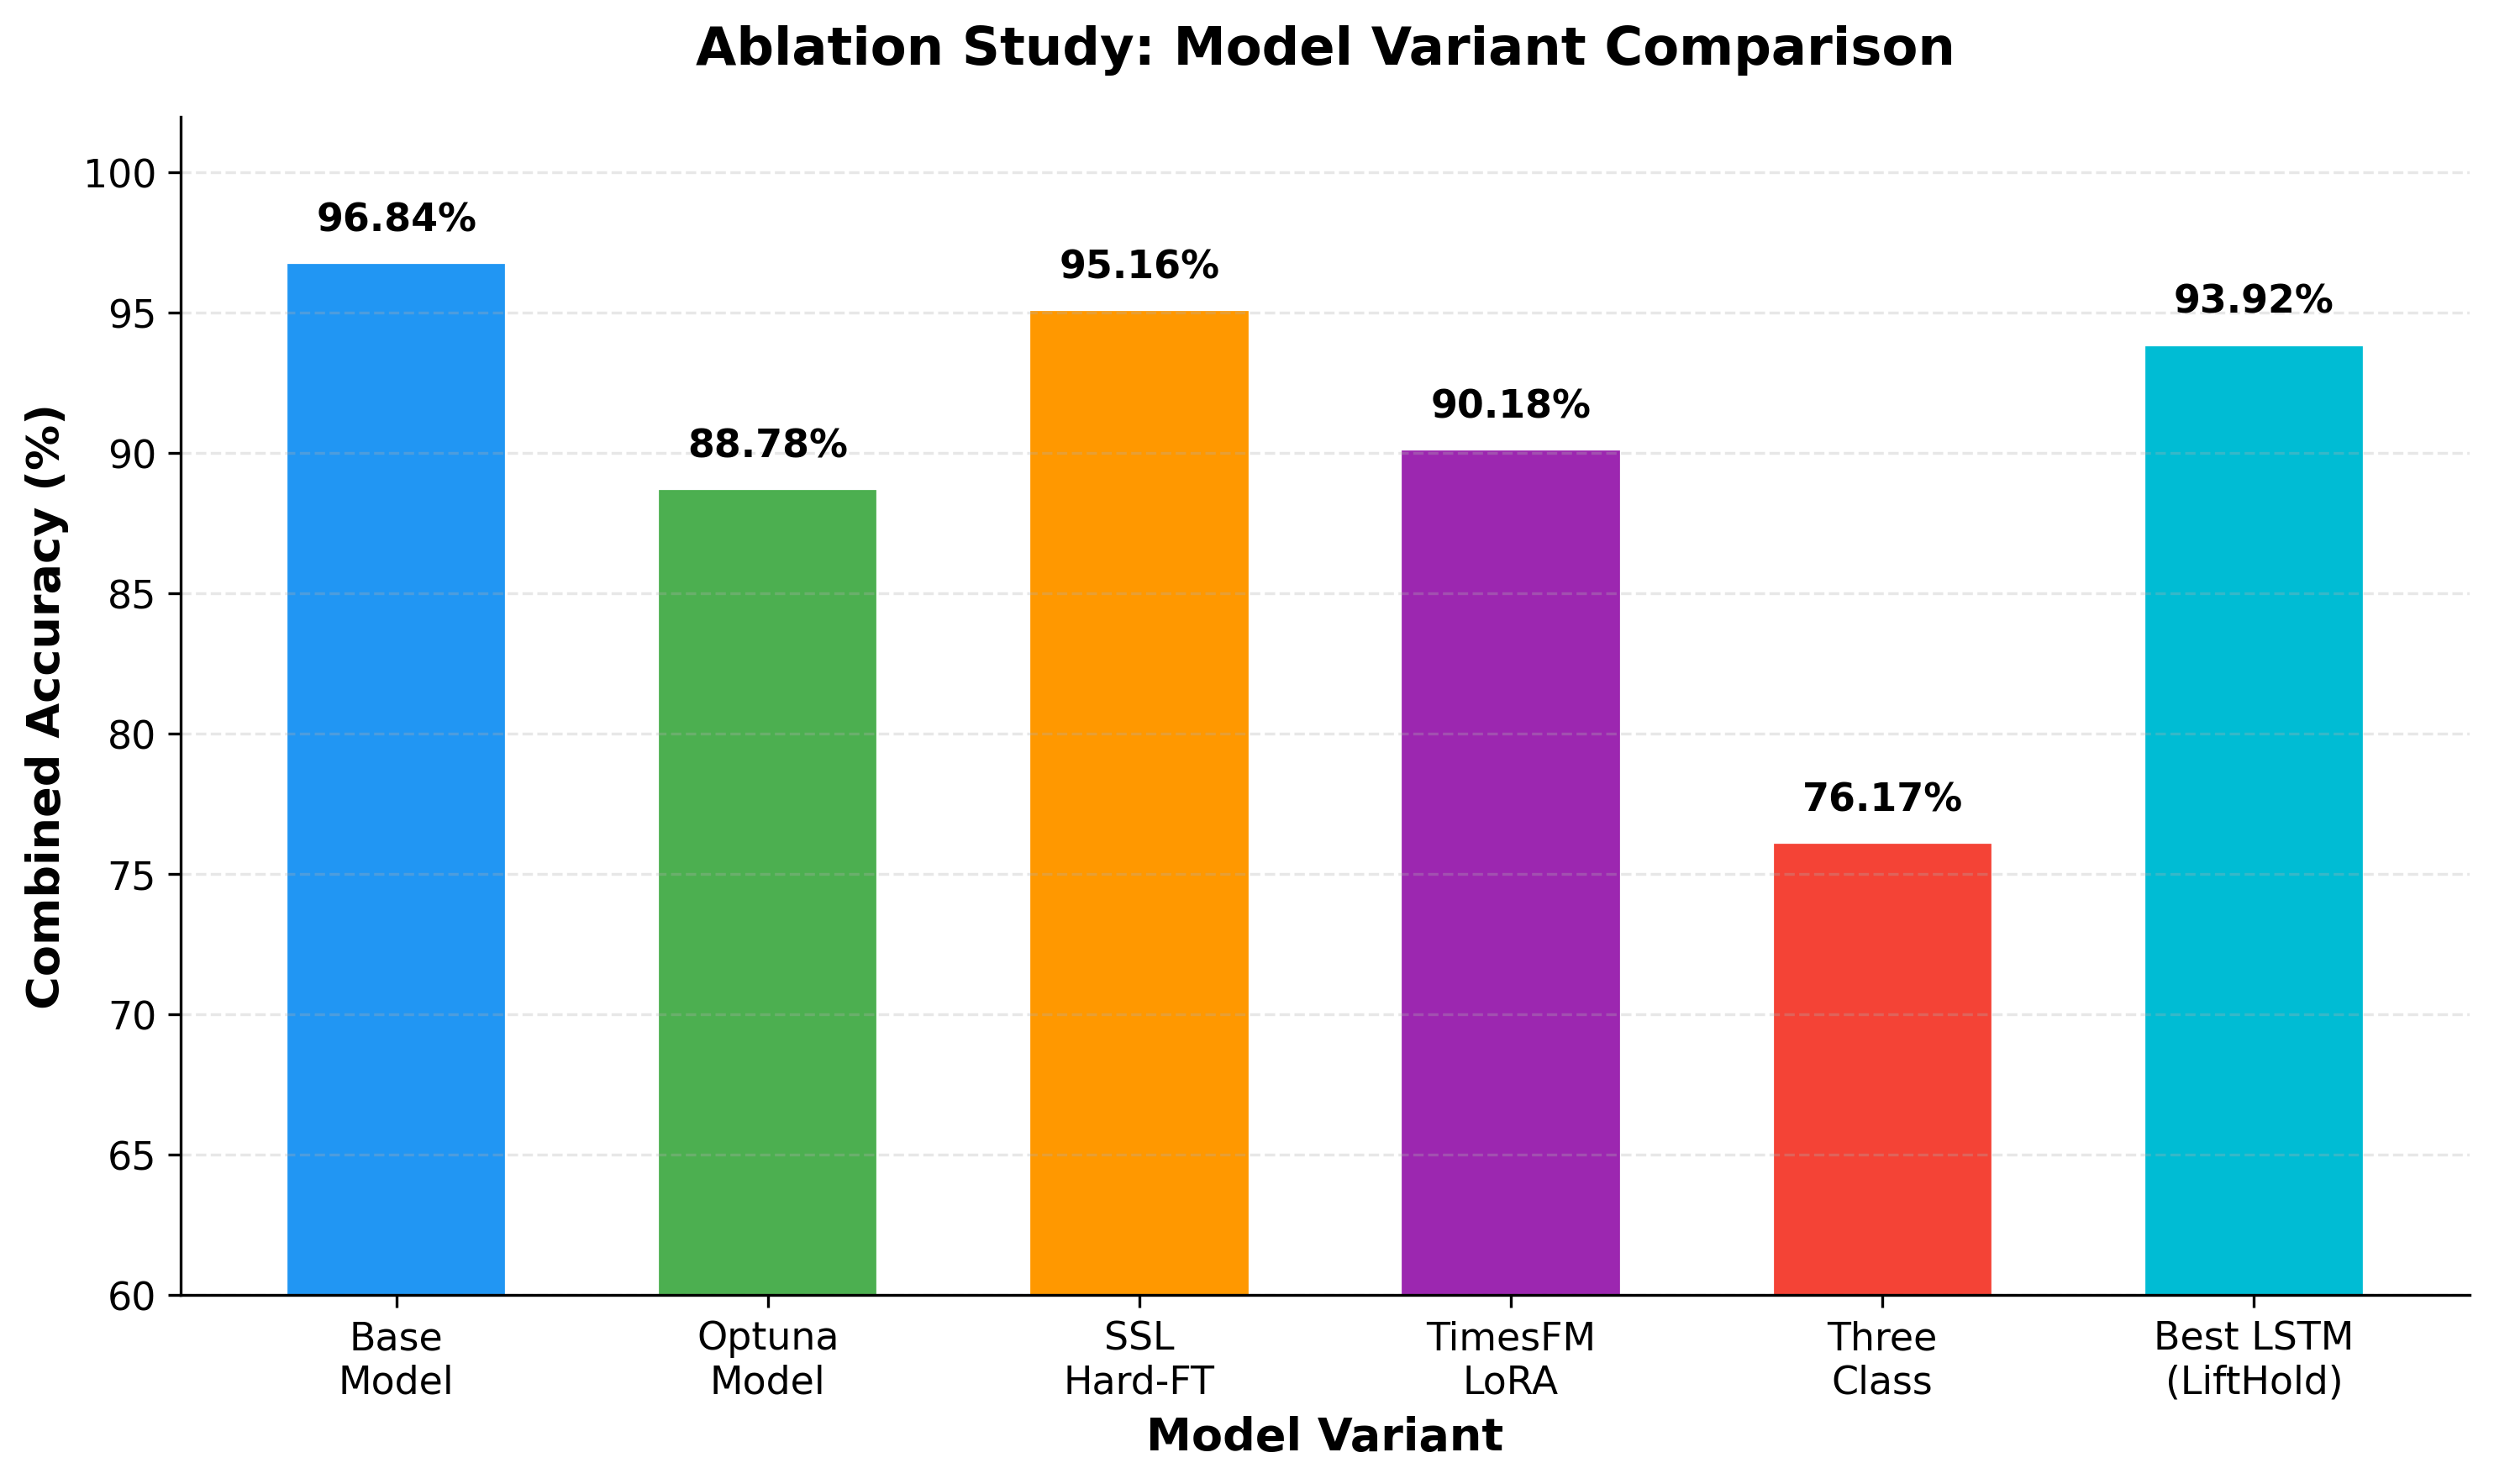
\includegraphics[width=0.45\textwidth]{plot_ablation_comparison.png}
\caption{Ablation comparison of combined accuracy across model variants.}
\label{fig:ablation}
\end{figure}


% ─── VIII. Conclusion ──────────────────────────────────────────────
\section{Conclusion}


% ─── Implementation Details ─────────────────────────────────────────
\section*{Implementation Details}

\begin{table}[H]
\centering
\begin{tabular}{ll}
\toprule
\textbf{Component} & \textbf{Detail} \\
\midrule
Framework             & PyTorch                                  \\
GPU environment       & CUDA-enabled GPU (Kaggle)                \\
Edge hardware         & Raspberry Pi (CPU)                       \\
HP optimisation       & Optuna (TPE sampler)                     \\
Signal processing     & SciPy (Butterworth filter, resampling)   \\
Gradient clipping     & Max norm $= 1.0$                         \\
LR scheduler          & ReduceLROnPlateau (factor $0.5$, patience $5$) \\
\bottomrule
\end{tabular}
\end{table}

% ─── References ─────────────────────────────────────────────────────
% \bibliographystyle{IEEEtran}
% \bibliography{references}

\end{document}
